\documentclass[a4paper,12pt]{article}

\usepackage{indentfirst}
\usepackage[utf8]{inputenc}
\usepackage{graphicx}
\usepackage{float}
\usepackage[portuguese]{algorithm2e}
\usepackage{amsmath}
\usepackage{xcolor}

\definecolor{pblue}{rgb}{0.13,0.13,1}
\definecolor{pgreen}{rgb}{0,0.5,0}
\definecolor{pred}{rgb}{0.9,0,0}
\definecolor{pgrey}{rgb}{0.46,0.45,0.48}

\usepackage{listings}
\lstset{language=Java,
	postbreak=\raisebox{0ex}[0ex][0ex]{\ensuremath{\color{red}\hookrightarrow\space}},
	showspaces=false,
	showtabs=false,
	breaklines=true,
	showstringspaces=false,
	breakatwhitespace=true,
	commentstyle=\color{pgreen},
	keywordstyle=\color{pblue},
	stringstyle=\color{pred},
	basicstyle=\tiny\ttfamily,
	moredelim=[il][\textcolor{pgrey}]{$$},
	moredelim=[is][\textcolor{pgrey}]{\%\%}{\%\%}
}
\title{Chat assíncrono criptografado utilizando  sockets TCP em Java}
\author{Sila Geroges Agiru Judick Siebert\\UDESC
        \and Wagner Luis Sousa da Luz \\UDESC}
\date{\today}


\begin{document}

\maketitle

\begin{abstract}
Neste artigo, uma aplicação de bate-papo para enviar mensagens  criptografadas é proposta.
O algoritmo de criptografia é caracterizado por inverter valor dos bits da mensagem. A aplicação é desenvolvida usando a linguagem de programação Java e utilizando sockets TCP. Este artigo resume as etapas de engenharia de software seguidas durante a implementação deste projeto.
\end{abstract}


\section{Introdução}
A maioria dos usuários de aplicativos de mensagens instantâneas convencionais na Internet não percebe que suas conversas estão sendo transmitidas em texto claro e são vulneráveis a espionagem durante a transmissão. 
\subsection{Objetivo}

O projeto foi intitulado  chat assíncrono criptografado e seu objetivo principal é implementar uma sala de bate-papo com criptografia nas mensagens. Objetivos secundarios foram a pesquisa sobre sockets e experiência prática dos autores no desenvolvimento de uma aplicação bate-papo baseada em Java utilizando conceitos de threads e sockets aprendidos em aula.

\subsection{Problema}
\subsubsection{Requisitos}
\begin{itemize}
\item a criptografia deve inverter valor dos bits da mensagem.
\item Devem utilizar uma conexão TCP/IP
\item não utilizar a classe bufferedreader e bufferedwriter
\end{itemize}


              
A figura \ref{fig1} representa uma sala de bate-papo.
\begin{figure}[H]
	\centering
	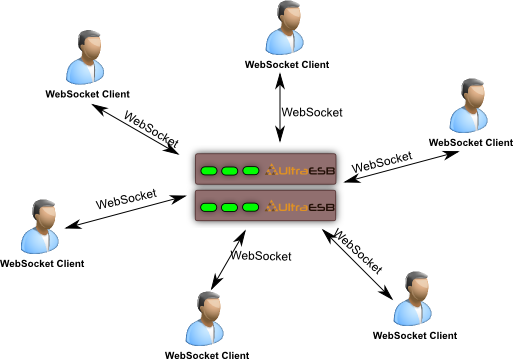
\includegraphics[scale=0.4]{img/454.png}    
	\caption{Sala de bate-papo}
	\label{fig1}     
\end{figure} 

\section{A sua Implementação}
\subsection{Diagramas}
\subsubsection{Diagramas de classe}
A figura \ref{fig2} representa o diagrama de classe da nossa implementação.
\begin{figure}[H]
	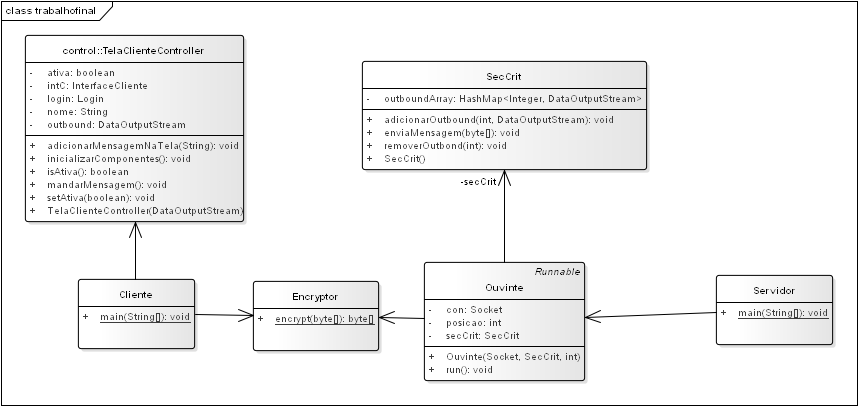
\includegraphics[scale=0.4]{img/class.png}    
	\caption{Class diagram}
	\centering
	\label{fig2}
	\end{figure} 
\subsubsection{Diagramas de atividade}
A figura \ref{fig3} representa o diagrama de atividade da classe servidor da nossa
implementação.
\begin{figure}[H]
\centering
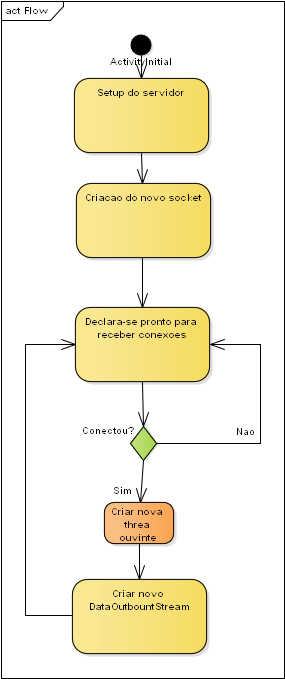
\includegraphics[scale=0.4]{img/serverflow.png}    
\caption{Activity diagram do servidor}

\label{fig3}
\end{figure}

\subsection{Codigo fonte}

\begin{figure}[H]
\lstinputlisting[firstline=8]{../../TrabalhoFinal/src/trabalhofinal/Servidor.java}
\caption{Codigo da classe Servidor}
\end{figure}

\begin{figure}[H]
\lstinputlisting[firstline=8,lastline=41]{../../TrabalhoFinal/src/trabalhofinal/Cliente.java}
\caption{Codigo da classe Cliente}
\end{figure}

\begin{figure}[H]
\lstinputlisting[firstline=16,lastline=23]{../../TrabalhoFinal/src/trabalhofinal/Encryptor.java}
\caption{Código da classe Encryptor}
\end{figure}


\section{Avaliação da implementação}
Durante a implementação algumas dificuldades forma surgindo. A primeira deles sendo como manter todas as mensagens sincronizadas e na ordem em todas as janelas de bate-papo.
Outra dificuldade identificada foi reenviar as mensagens enviados de um cliente para o servidor, para todos os outros clientes.
A ultima dificuldade foi implementar a criptografia. Para isto algumas estrategias foram tentadas, nenhuma funcionando ate finalmente trabalhar somente com vetores de bytes.
\section{Conclusão}
Síntese do que foi dito.\\
Lista dos resultados atingidos:
\begin{itemize}
\item resultado 1
\item resultado 2 e teste de bibliografia \cite{Bulfinch1998}
\end{itemize}
Conclusão final e Trabalho Futuro.

\bibliographystyle{plain}
\bibliography{n2library.bib}

\end{document}
